\documentclass[report]{BetterDocument}

\title{Méthode de conception}
\subtitle{Création d'un jeu d'assemblage}
\author{Justine MARTIN 21909920}
\date{2020 - 2021}
\institute{Unicaen}

\instituteLogo{img/unicaen.png}
\docLogo{}

\begin{document}

	\pageDeGarde

	\section{Les choix technologiques}

		Pour ce projet, j'ai fait le choix d'utiliser Gradle, outil que j'ai déjà pu réutiliser à de très nombreuses reprises, plutôt que Ant car il possède de nombreux avantages par rapport à ce dernier. En voici quelques exemples :

		\begin{itemize}
			\item{La gestion du projet est beaucoup plus clair et simple qu'avec un fichier xml}
			\item{La gestion des modules est beaucoup plus simple}
			\item{On peut utiliser des dépots de maven pour les dépendences}
			\item{La communauté y est grande. C'est notamment le moteur de production utilisé par Google pour les projets Android}
		\end{itemize}

	\section{Les modules}

		Tout d'abord, il faut rappeller que notre jeu n'est pas le seul à utiliser un système de pièce de cette manière. En effet, Tétris en est un bon exemple. Là où Tétris diffère de notre jeu c'est, par exemple, qu'il existe une translation des pièces vers le bas à interval régulier. La génération d'une grille n'est pas la même non plus, tout comme le calcul de score qui est spécifique à notre application.

		Suivant ce principe, j'ai alors décidé que la lib \textit{piecesPuzzle} devrait contenir un code qui peut être suffisement général pour être réutilisé par un autre projet, ici, il s'agit de \textit{jeuAssemblage}. Ainsi, toujours suivant le même principe, tous les principes / classes spécifiques seront stockés dans le projet \textit{jeuAssemblage} (tel que le calcul du score, la génération du plateau, les règles du jeu, ...).

	\section{Gestion des pièces}

		\subsection{Représentation d'une pièce}

			Concernant la gestion des pièce, une classe mère nommée \textbf{AbstractPiece} contient tout le code commun aux pièces. Comme son nom l'indique, celle-ci est abstraite et ne définit que le comportement commun à chaque pièce (taille, rotation, position, ...).

			Chaque pièce est représentée par un tableau de boolean de taille $largeur * hauteur$. Si une case de celui-ci vaut \textit{true}, alors la case est pleine, sinon, elle est vide. Ce tableau est complètement figé et n'est pas affecté par la rotation. La sous partie suivante détaillera la gestion des rotations.

			Chaque classe fille de \textbf{AbstractPiece} doit redéfinir la méthode \textit{boolean[] generatePiece(int w, int h)} afin de retourner le tableau de boolean qui représente la pièce. On a ici un "pattern template" comme on peut le voir sur la figure \ref{fig:pattern_template}

			\begin{figure}[H]
				\centering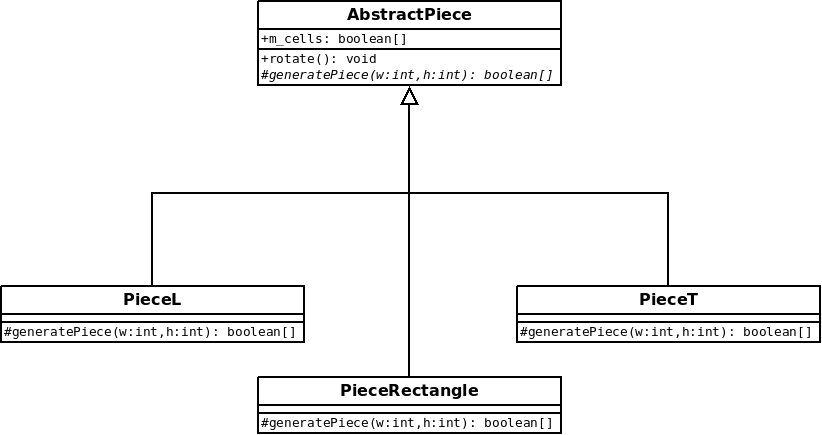
\includegraphics[width=0.65\textwidth, keepaspectratio]{img/pattern_template.png}
				\caption{Le pattern template}
				\label{fig:pattern_template}
			\end{figure}

		\subsection{Rotation d'une pièce}

			Concernant la méthode utilisée pour la rotation des pièces, j'ai décidé d'utiliser un compteur que j'incrémente à chaque rotation. Ainsi, lorsque j'incrémente le compteur, une rotation dans le sens horraire se fait et lorsque je le décrémente, une rotation dans le sens anti-horaire se fait. Comme dit précédemment, le tableau ne change pas ce qui permet de limiter le nombre de \textit{new}. La rotation est cependant prise en compte lorsque l'on demande si une case est remplis ou non. En effet, on va appliquer aux coordonnées x y de la case demandé le nombre de rotation effectué mais dans le sens inverse (anti-horaire donc) afin d'obtenir la case demandé sur le tableau de la pièce sans rotation.

			On vérifie d'abord que la coordonnée souhaité ne sors pas de la pièce :

			\begin{lstlisting}[gobble=16, language=Java, caption=Vérification pré rotation]
					if(x < 0 || x >= getWidth()) {
						return false;
					} else if(y < 0 || y >= getHeight()) {
						return false;
					}
			\end{lstlisting}

			On continue ensuite en bouclant afin d'appliquer le nombre de rotation correct. La méthode est simple, une rotation échange la largeur et la hauteur d'une pièce. De même pour les composantes x et y. Elle s'echangent à ceci prêt que $y$ devient $-x + largeur - 1$. De ce fait, on obtient la boucle suivante :

			\begin{lstlisting}[gobble=16, language=Java, caption=Inversement du nombre de rotation]
				for(int i = m_rotationCount ; i % 4 != 0 ; i--) {
					int tmp = pieceX;
					pieceX = pieceY;
					pieceY = -tmp;

					// On remonte la pièce
					pieceY += ((i % 2 == 0) ? m_width : m_height);
					pieceY -= 1;
				}
			\end{lstlisting}

			Enfin, il ne reste qu'a retourner la valeur de la case :

			\begin{lstlisting}[gobble=16, language=Java, caption=Retourne la valeur de la case]
				return m_cells[pieceX + pieceY * m_width];
			\end{lstlisting}

	\section{Actions}

		Afin d'interagir sur le plateau on utilise des actions, normalisés par l'interface \textbf{IAction}. Celle-ci défini deux méthodes. La première, \textit{boolean isValid()} détermine si l'action est valide, c'est a dire possible. La seconde \textit{void apply()} se charge d'appliquer l'action. Il est très important de les utiliser car c'est elles qui notifient les listeners qu'une action est survenue sur le plateau.

		On obtient alors le diagramme suivant (seul deux classes filles sont représentées) :

		\begin{figure}[H]
			\centering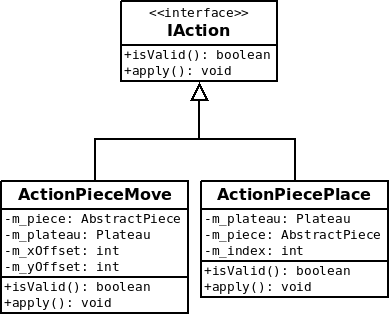
\includegraphics[width=0.4\textwidth, keepaspectratio]{img/action.png}
			\caption{Diagramme de classe concernant les actions}
		\end{figure}

		Ce système permet de séparer correctement le code tout en allégeant celui du plateau car les traitement complexes et lourds à lire se retrouvent dans une classe à part. Ainsi, pour utiliser une action il s'uffit d'utiliser un code tel que celui-ci :

		\begin{lstlisting}[gobble=12, language=Java, caption=Utilisation d'une Action]
			IAction action = new ActionPieceRotate(plateau, piece);
			if(action.isValid())
				action.apply();
		\end{lstlisting}

	\section{Quelques pattern}

		\subsection{M/VC}

			Bien entendu, le pattern MVC à été implémenté pour la classe \textbf{Plateau} ainsi que pour \textbf{GameState}, classe qui représente l'état actuel du jeu. De ce fait, on a donc la mise en place d'un pattern observer. La mise en place de ce pattern s'est fait de la manière suivante :

			\begin{figure}[H]
				\centering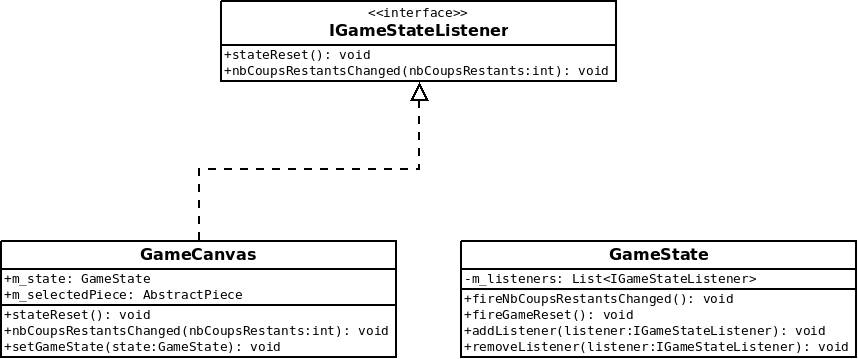
\includegraphics[width=0.65\textwidth, keepaspectratio]{img/mvc.png}
				\caption{MVC sur le GameState}
			\end{figure}

			Notre \textbf{GameCanvas} possède l'instance actuelle de \textbf{GameState} dans le cas où l'on utilise le setter pour modifier cette instance, on met à jour la liste des listeners. A chaque fois que l'on va reset ou changer le nombre de coups restants dans la classe \textbf{GameState}, on va utiliser la méthode fireXXX approprié. On va alors parcourir la liste des listeners pour les notifier du changement et leur demander de faire les actions adéquates. Dans le cas de GameCanvas, le seul cas qui nous intéresse est celui où l'etat du jeu est remis à 0 car il faut alors redessiner le plateau.

		\subsection{Pattern Factory}

			La génération d'une pièce aléatoire se fait par l'utilisation d'une Factory, \textbf{PieceFactory} dans la librairie \textit{piecesPuzzle} grace à la méthode statique \textit{AbstractPiece generatePiece()}. Cette méthode va alors tirer des nombres au hasard pour choisir la pièce. Trois autres nombre sont alors tirés afin de déterminer la largeur, la hauteur et enfin le nombre de rotations. Une fois que la pièce est générée, on la retourne. Il faut bien noter que la méthode ne sélectionne pas de position de départ à celle ci car la position est très liée à la taille de la grille. De plus, la position de sortie est aussi lié au type de jeu que l'on souhaite faire. Dans un Tétris, la pièce serait placée tout en haut au milieu tandis que dans notre jeu, la pièce peut être placée n'importe où sur la grille.

		\subsection{Pattern strategy}

			Le pattern strategy a été utilisé à de très nombreux endroit. Il l'a été dès qu'une méthode ou une technologie particulière a été utilisée. C'est par exemple le cas pour l'export et l'import d'une partie, la génération du plateau, le calcul du score, ... Cela permet d'intégrer très facilement une nouvelle manière de gérer ces élément sans pour autant devoir réécrire une bonne partie du code car le fonctionnement se retrouve formalisé dans les grandes lignes. En voici un exemple concernant l'import et l'export d'une partie :

			\begin{figure}[H]
				\centering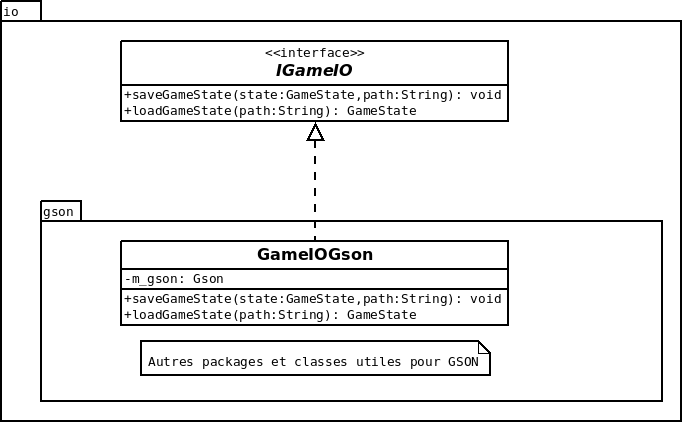
\includegraphics[width=0.65\textwidth, keepaspectratio]{img/pattern_strategy.png}
				\caption{Pattern strategy pour l'import et l'export d'une partie}
			\end{figure}

	\section{Tests unitaires}

		Pour les tests unitaires j'ai décidé d'utiliser JUnit et Mockito. Ce dernier sert à mocker très facilement des objets et obtenir pas mal d'outils de vérification supplémentaire (nombre d'appel à une méthode par exemple).

		J'ai surtout préféré me concentrer sur les tests concernant la librairie car il s'agit de la partie la plus simple et la plus importante à tester. Chaque méthode qui nécessite un traitement un peu particulier dans son code à ainsi été testée. Le plus important étant de tester le plus de cas possibles. Voici un exemple de test réalisé afin d'expliquer un peu plus Mockito qui n'a pas été vu en cours :

		Nous allons tester la classe ActionPipeline qui permet d'exécuter plusieurs actions suite à suite. On doit tout d'abord commencer par préciser à JUnit que l'on doit utiliser le Runner de Mockito grace à l'annotation \textit{@RunWith} auquel on passe le type \textbf{MockitoJUnitRunner}. On peut alors annoter les objets que l'on souhaite mocker avec \textit{@Mock}. Ici nous allons mocker deux actions.

		\begin{lstlisting}[gobble=12, language=Java, caption=Exemple de mock avec mockito]
			@RunWith(MockitoJUnitRunner.class)
			public class TestActionPipeline {
				@Mock
				private IAction m_action1;

				@Mock
				private IAction m_action2;

				// [...]
			}
		\end{lstlisting}

		Mockito permet de spécifier ce que doit retourner un objet en cas d'appel à une de ses méthodes. Par exemple, \textit{m\_action1} va ici retourner true lorsque que l'on fera un appel à \textit{isValid()} grace à la ligne\\ \textit{Mockito.when(m\_action1.isValid()).thenReturn(true)}. On peut ensuite s'assurer du résultat de la pipeline avec un \textbf{Assert} comme c'est le cas habituellement. Enfin, on peut s'assurer que les méthodes on bien été apellées grace à la ligne \textit{Mockito.verify(m\_action1, Mockito.times(1)).isValid()}. Ici, on s'assure que la méthode \textit{isValid()} a bien été appellé 1 fois.

		\begin{lstlisting}[gobble=12, language=Java, caption=Exemple de test avec mockito]
			@Test
			public void isValid() {
				ActionPipeline pipeline = new ActionPipeline();
				pipeline.addAction(m_action1);
				pipeline.addAction(m_action2);

				// Mock le résultat de isValid
				Mockito.when(m_action1.isValid()).thenReturn(true);
				Mockito.when(m_action2.isValid()).thenReturn(true);

				Assert.assertTrue(pipeline.isValid());

				// On vérifie que isValid a été call sur les deux IActions
				Mockito.verify(m_action1, Mockito.times(1)).isValid();
				Mockito.verify(m_action2, Mockito.times(1)).isValid();

				// On change le premier Mock
				Mockito.when(m_action1.isValid()).thenReturn(false);

				Assert.assertFalse(pipeline.isValid());

				// On vérifie que le isValid du premier mock a été call une fois de plus et pas l'autre
				Mockito.verify(m_action1, Mockito.times(2)).isValid();
				Mockito.verify(m_action2, Mockito.times(1)).isValid();
			}
		\end{lstlisting}

	\section{Liste de points améliorable}

		Bien sûr le code est loin d'être parfait, voici une liste non exhaustive des points que j'aurai souhaité améliorer :

		\begin{itemize}
			\item{La \textbf{PieceFactory} devrait complètement gérer la création des pièces et sauvegarder le tableau généré dans un tableau. Ainsi, si on demande deux fois de générer une pièce en T de 3 de largeur et 5 en hauteur, le tableau ne sera généré qu'une seule fois}
			\item{L'utilisation des \textbf{Actions} ne me plait pas. J'aurais aimé que chaque actions soit instancié en dehors de la classe \textbf{Plateau} ou \textbf{AbstractPiece} et qu'elle appelle une méthode de ces dernières (ce n'est pas le cas pour l'ajout d'une pièce sur le plateau actuellement)}
			\item{Il n'y a pas de test unitaire sur la partie \textit{jeuAssemblage}}
			\item{La génération du plateau ne permet pas forcément de faire un rectangle sans case vide}
			\item{Utilisation de factory pour générer une instance d'une classe qui est basé sur le Pattern strategy. Une constante définirait la classe fille a utiliser. Le changement de classe fille serait donc plus facile et ne nécessiterai plus de rechercher dans le code les différents instanciations d'une classe}
		\end{itemize}

\end{document}
